\section{Background} 
\label{sec:bg}
In this section we give a brief overview of DRAM, covering the organization, basic operation, refresh modes, and trends together with projections for the DRAM structure.

DRAM is hierarchically organized as in \reffig{fig:dram_orga}. At the top of the hierarchy are the \textit{channels} that are connected to one or more \textit{ranks}, each composed of multiple storage arrays called \textit{banks}. Each channel has individual address, data, and command buses that makes it possible for the channels to operate concurrently. All ranks on one channel can operate in parallel, but are constrained by the channel bandwidth, which is shared among the ranks. Further, the banks within the ranks operate in parallel, but are constrained by both the shared channel bandwidth and resources shared among the banks. 

The DRAM cell array in each bank is structured as in \reffig{fig:dram_orgb}. One cell consists of a transistor and a capacitor, where the transistor is controlled by the \textit{word line} wire and connects the capacitor to the \textit{bit line} wire. The word line connects a number of cells which forms a row. Each bit line is connected to a sense amplifier, and the row of sense amplifiers constitutes the \textit{row buffer}. Data is stored as a charge on the cell capacitor.

\begin{figure*}[t]
    \centering
    \subfigure[DRAM hierarchy]{
        \centering
        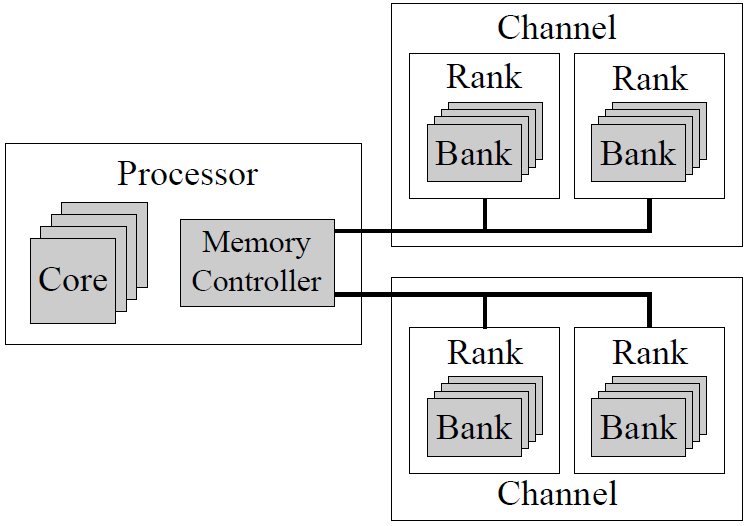
\includegraphics[width=0.4\textwidth]{dram_orga}
		\label{fig:dram_orga}
    }
    \subfigure[DRAM bank structure]{
        \centering
        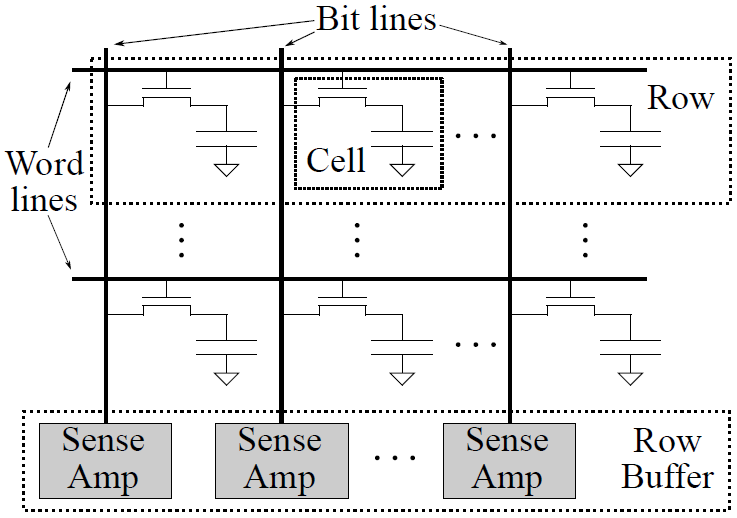
\includegraphics[width=0.4\textwidth]{dram_orgb}
		\label{fig:dram_orgb}
    }
	\caption{DRAM system organization \cite{raidr}.}
	\label{fig:dram_org}
\end{figure*}

To read a row, the word line connected to the row's transistors must first be activated. When the word line is activated, the transistors connect the capacitors to the bit lines. When the capacitors connect to the bit lines, charge will either flow from or to the capacitors depending on whether they were charged or not, respectively. For this to work, the bit lines have to be precharged to $V_{DD}/2$. The sense amplifiers then detect the change of voltage, which makes it possible to interpret the stored data. The charge stored on the capacitors has, as mentioned, left the capacitor and a read operation is thus destructive. To maintain the data the capacitors are recharged by the bit lines, which are driven to either either $V_{DD}/2$ or $0\:V$ by the sense amplifiers depending on the former voltage detected. Finally, when another row on the bank is accessed, the open row has to be closed, which disconnects the capacitors from the bit lines.

To write to a row, the corresponding word line is first activated. As during a read, the transistors then connect the capacitors to the bit lines, and charge will either flow from or to the capacitor. The row buffer is then loaded with the data that are driven to the bit lines by the sense amplifiers, thus storing the information on the capacitors. The row will be closed when another row is accessed.

As mentioned, the capacitors leak charge over time and have to be recharged in order to preserve the data. The refresh is performed by opening a row to let the sense amplifiers magnify the detected voltage change and thus recharge the cells to either $V_{DD}/2$ or $0\:V$. This follows the same procedure as a read operation and thus is the row always refreshed when a read is performed. % Is it clear that the row is refreshed during a write?

The memory controller (MC) normally issues refresh operations periodically at an interval of $64\:ms$ for each row, an interval that has been constant for the latest DRAM specifications [source] and called \textit{maximum refresh period}. This interval is conservatively halved if the DRAM exceeds the specified working temperature of $85^{\circ}C$. 

To refresh one rank, the simplest approach is to refresh all banks in parallel row-by-row at the start of the $64\:ms$ interval. This approach is called \textit{burst refresh}. The approach blocks normal accesses for a long period, and power consumption peaks during the burst time. A better alternative is to use \textit{distributed refresh}, which scatter the refreshes across the interval, resulting in a lower average latency for the processor and more stable power consumption.

The implementation of a DRAM refresh cycle can be made in two different ways, to either affect one row or many. The first is called \textit{RAS-only refresh} (ROR) where a refresh cycle refreshes one targeted row. To target one row, the row's address is put on the bus, and the MC have the responsibility that a row is refreshed within the maximum refresh period. The second is called \textit{CAS before RAS refresh} (CBR). In this scheme, the memory module have an internal address counter that displays which row that will be refreshed. On a refresh cycle, the row stated by the internal address counter is refreshed and the counter is then incremented. Contrary to ROR, CBR do not need provided addresses on the bus, which results in a lower power consumption and less bus usage. % During CBR, a row in each bank is updated, right? if so. write that in the text.

When using CBR, all banks in a rank are blocked for normal accesses. All banks are also blocked when ROR is used due to DRAM chip design, however some DRAM chips support per-bank refresh commands that makes it possible to only block the specific bank being refreshed. 

\begin{figure}[t]
    \centering
    \subfigure[DRAM throughput loss]{
        \centering
        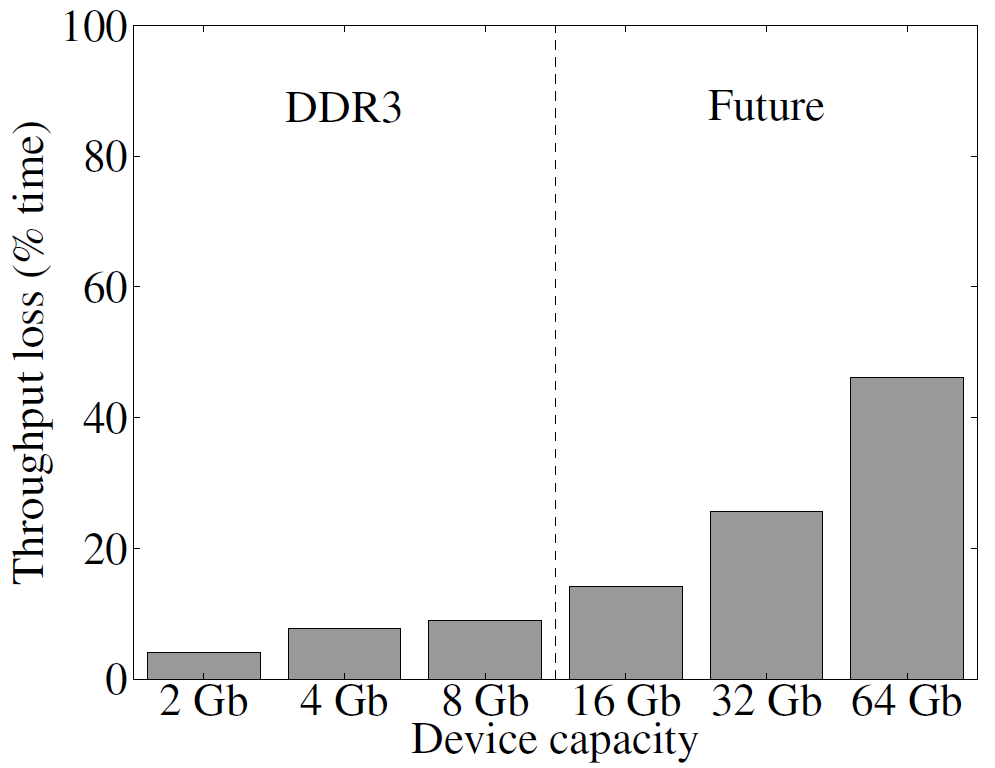
\includegraphics[width=0.33\textwidth]{dram_throughput}
        \label{fig:dram_throughput}
    }
    \subfigure[DRAM power consumption]{
        \centering
        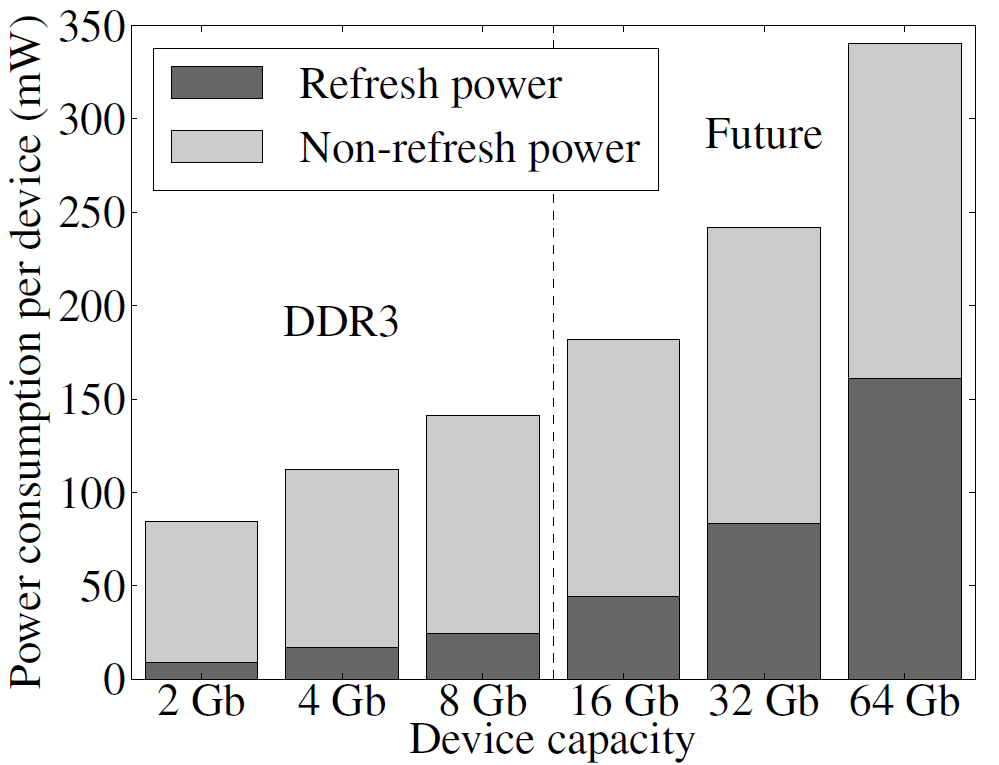
\includegraphics[width=0.33\textwidth]{dram_power}
        \label{fig:dram_power}
    }
    \caption{Projections on DRAM throughput loss and power consumption in extended-temperature operation \cite{raidr}.}
    \label{fig:dram_data_proj}
\end{figure}

The trends in DRAM chips is to increase capacity with each generation. In practice, this is realized to a high degree by adding additional rows in the banks. The rows could instead - or also - been made longer by adding DRAM cells, but this solution is not favorable as it increases the power consumption per row access. 

As refresh operations are made by row, the refresh operations will increase linearly with the device capacity. In turn, the throughput loss increases exponentially, as shown in \reffig{fig:dram_throughput}. Additional refresh operations give larger power consumption and the refreshes become a growing portion of the total DRAM energy consumption, as shown in \reffig{fig:dram_power}. When the device capacity reaches $64\:GB$, the refresh power nearly constitutes half of the total consumption, an increase from 15\% if the device capacity is 8 GB. 

The conclusion to draw from \reffig{fig:dram_data_proj} is that it will be increasingly important to mitigate the throughput loss and DRAM power consumption of future systems. One way to decrease these negative trends of DRAM scaling is to optimize the DRAM refresh. However, a reduction in the number of refreshes made has no linear relationship to the reduction in refresh energy consumption. The energy reduction depends on the state of the bank in which the targeted row resides; if the targeted row is closed more energy will be consumed than if the targeted row would have been open.